%############################################################################
\section{User Interface}
\label{sec:ap-interface}
%############################################################################

\AutoProof is available in two modes of operation: (1) through a graphical interface integrated in the \EVE IDE and (2) as a command-line tool. In addition, there are two different web interfaces that gives access to the command-line version of \AutoProof, each with different limitations.


%============================================================================
\subsection{\AutoProof in \EVE}
%============================================================================

\EVE is the Eiffel Verification Environment, an Eiffel IDE based on EiffelStudio~\cite{EIFFELSTUDIO}. \EVE contains various research tools including \AutoProof. In \EVE, \AutoProof is available as a separate tool panel. Figure~\ref{fig:eve-tool-panel} shows EVE with the \AutoProof panel open in the bottom left. 

\begin{figure}[ht]
\centering
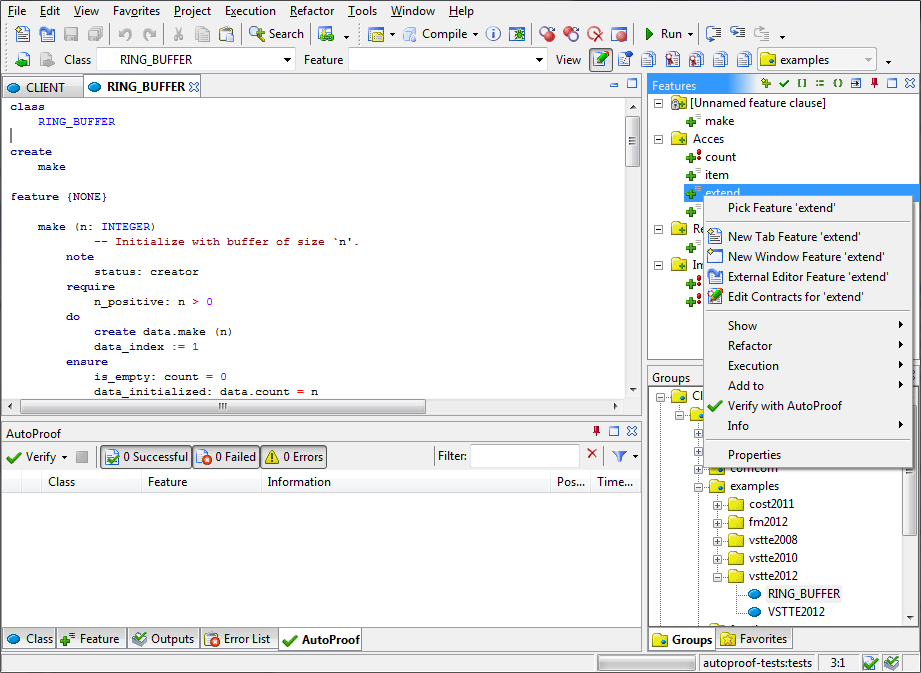
\includegraphics[width=\textwidth]{images/eve_layout_with_context_menu.png}
\caption{The \AutoProof tool panel in \EVE (lower left) and the context menu of a feature (right side).}
\label{fig:eve-tool-panel}
\end{figure}

%----------------------------------------------------------------------------
\subsubsection{Running \AutoProof}
%----------------------------------------------------------------------------

The scope of the input to \AutoProof can be selected by interacting with the \emph{Verify} button:
\begin{itemize}
\item \emph{Verifying a single feature}: pick-and-drop a feature on the button.
\item \emph{Verifying a single class}: either open a class in the editor and click the button or pick-and-drop a class on the button.
\item \emph{Verifying all classes in a cluster or library}: either open a cluster in the editor and click the button, pick-and-drop a cluster or library on the button, or use the drop-down arrow on the button to verify the cluster the currently selected class is in.
\item \emph{Verifying the whole system (excluding libraries)}: use the drop-down arrow on the button and select \emph{Verify System}
\end{itemize}

The user can also right-click any feature, class, cluster, or library and select the \emph{Verify with \AutoProof} option from the context menu (see right side of Figure~\ref{fig:eve-tool-panel}).

\AutoProof will always check that the system compiles successfully with the Eiffel compiler before starting the verification. This ensures that the code that is verified is valid Eiffel code. Only one instance of \AutoProof can run at the same time, so during the execution of \AutoProof the \emph{Verify} button is disabled while the red \emph{stop} button next to it is enabled. With the stop button the user can abort a long-running verification if necessary.



%----------------------------------------------------------------------------
\subsubsection{Displaying results}
%----------------------------------------------------------------------------

\begin{figure}
\centering
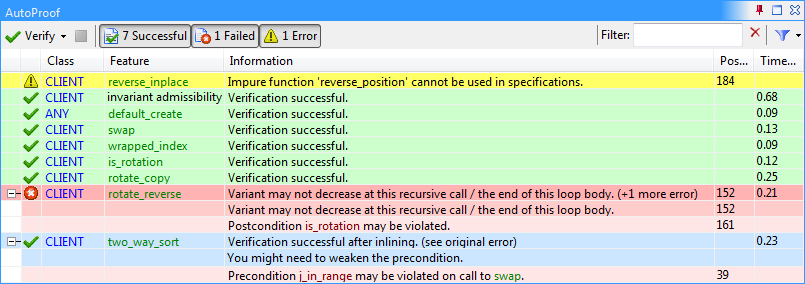
\includegraphics[width=\columnwidth]{images/eve_panel_results.png}
\caption{The \AutoProof panel showing the results of a verification.}
\label{fig:eve-tool-result}
\end{figure}

After the verification is finished, \AutoProof displays the results of the verification in the tool panel. It displays the verification result for each individual routine separately. Figure~\ref{fig:eve-tool-result} shows an example of running \AutoProof. There are four possible outcomes per routine:
\begin{itemize}
\item \colorbox[HTML]{CCFFCC}{Green row:} The verification was successful.
\item \colorbox[HTML]{FFBBBB}{Red row:} The verification failed. An error message will indicate what type of assertion was not verified correctly and, if possible, indicate the assertion tag and line number of the assertion. It is also possible that there are multiple violations for a single routine in which case the row can be expanded to show all messages.
\item \colorbox[HTML]{FFFF66}{Yellow row:} There was invalid input to \AutoProof and the verification of that routine was not possible. This usually means an Eiffel construct is present that \AutoProof does not support or an Eiffel assertion is invalid in another way (e.g. an impure function is used in a contract).
\item \colorbox[HTML]{DDEEFF}{Blue row:} The verification was successful in the second step of two-step verification. The row can be expanded to show a possible suggestion of what the user can do to fix the original problem as well as the message of the failed first verification step.
\end{itemize}

In addition to the information about the routine and the message, the row will also indicate how long it took Boogie to verify that particular routine. The Eiffel elements such as class and feature names and the line number (if available) can be used to jump to the respective source location.

%----------------------------------------------------------------------------
\subsubsection{Verification options}
%----------------------------------------------------------------------------

The user can change the behavior of \AutoProof by enabling or disabling the following options:

\begin{itemize}
\item \emph{Two-step verification}: if enabled, a second verification attempt will be made on failed verifications.
\item \emph{Automatic inlining of routines}: if enabled, routines without postconditions will be automatically inlined.
\item \emph{Automatic loop unrolling}: if enabled, loops without a loop invariant will be automatically unrolled.
\item \emph{Generate postcondition predicates}: If enabled, \AutoProof will generate postcondition predicates and corresponding axioms to verify polymorphic calls.
\item \emph{Overflow checks}: if enabled, \AutoProof will check arithmetic operations for overflows.
\item \emph{Generate triggers}: if enabled, \AutoProof will generate triggers for quantified arithmetic expressions in Boogie.
\item \emph{Bulk or forked verification}: the user can choose between verifying all routines in one Boogie execution or running Boogie on each routine individually.
\end{itemize}


%============================================================================
\subsection{\AutoProof on the Command-line}
%============================================================================

Using \AutoProof on the command-line is similar to using the regular Eiffel compiler. In addition to specifying the Eiffel project, the user has to specify the \emph{-autoproof} option to launch \AutoProof after the Eiffel compilation succeeded. To set options of \AutoProof such as enabling or disabling arithmetic overflow checks, the user can add additional command-line flags for \AutoProof (see Appendix~\ref{manual:options} for details). Lastly, the user can also specify which classes and routines should be verified. If no selection is given, the whole system (excluding libraries) will be verified. The following command shows an example of launching \AutoProof with the project file \e{lcp.ecf} and overflow checking enabled on the single routine \e{LCP.client}:

\begin{lstlisting}[language=bash]
ec.exe -config lcp.ecf -autoproof -overflow LCP.client
\end{lstlisting}

The output of the verification will be printed to the console analogous to the graphical version of \AutoProof.


%============================================================================
\subsection{\AutoProof on the Web}\label{sec:ap:webui}
%============================================================================

There are two web-interfaces available for \AutoProof: (1) Comcom~\cite{APCOMCOM} and (2) E4Pubs~\cite{APE4PUBS}. Both of them can be used to deploy examples, provide an online editor to change the examples, and can run \AutoProof on the examples using the command-line interface of \AutoProof. There are different limitations and use cases though.

%----------------------------------------------------------------------------
\subsubsection{Comcom}
%----------------------------------------------------------------------------

\begin{figure}[p]
\centering
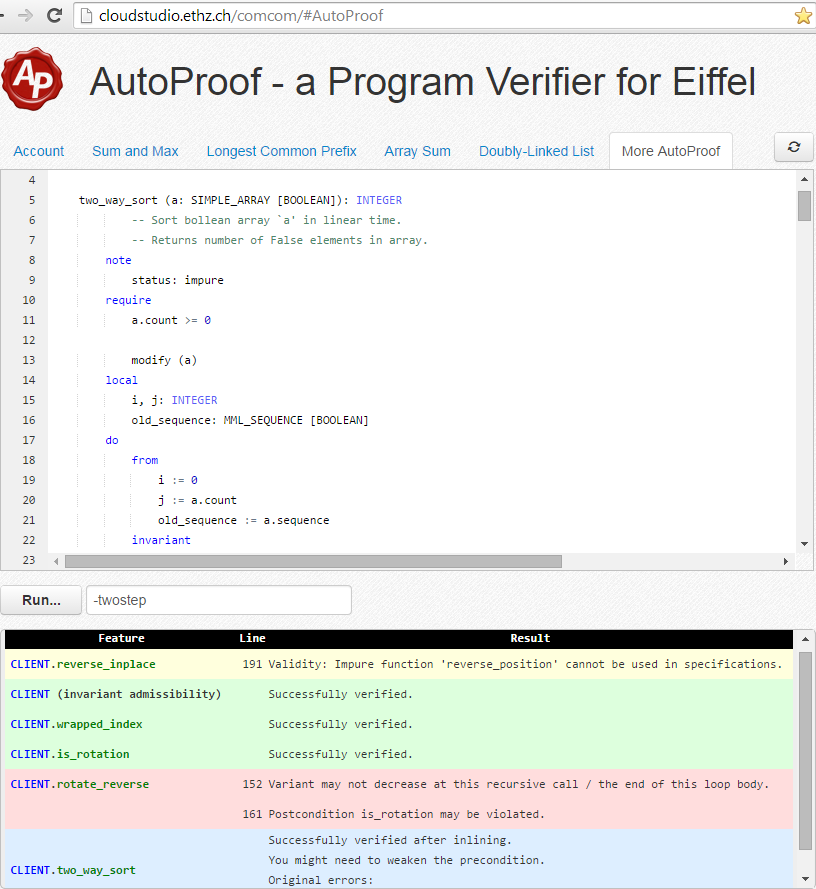
\includegraphics[width=\columnwidth]{images/comcom_screenshot.png}
\caption{Screenshot of comcom after running an example.}
\label{fig:ap-comcom}
\end{figure}

\emph{Comcom} is a web-interface for command-line tools. It features a list of predefined examples that the user can choose and modify as well as the possibility to write custom code from scratch and provide command-line arguments to \AutoProof. 
Figure~\ref{fig:ap-comcom} shows the interface of Comcom after running an example verification.

The limitation of \AutoProof on Comcom is the use of single-file examples. Since Eiffel only allows one class per file, the examples on Comcom have to be self-contained in one class. The user can use any class from the Eiffel base library, so it is still possible to write interesting examples and algorithms.

Due to Comcom's integration with the \emph{rise4fun} API, \AutoProof is also available on the rise4fun website~\cite{APRISE4FUN}.

%----------------------------------------------------------------------------
\subsubsection{E4Pubs}
%----------------------------------------------------------------------------

The second web-interface to \AutoProof is \emph{E4Pubs}, which stands for \emph{Eiffel 4 Publications}. It offers to host a predefined set of examples that can be verified with \AutoProof. Each example can---in contrast to---contain multiple classes. On the other hand, there is no possibility to write a custom example from scratch or provide command-line arguments. This web-interface is used to host examples for publications or to showcase features of \AutoProof, as each example has a unique URL and the examples can also be embedded in other websites. We use E4Pubs for example to create an interactive tutorial for \AutoProof~\cite{APTUTORIAL} and showcase benchmark examples~\cite{APREPO}.



